\documentclass[12pt]{article}
\usepackage[utf8x]{inputenc}
\usepackage[usenames,dvipsnames,svgnames]{xcolor}
\usepackage{amsmath}
\usepackage{graphicx}
\usepackage{float}
\usepackage{dsfont}
\usepackage{amsfonts}
\usepackage[T1]{fontenc}
\usepackage[colorinlistoftodos]{todonotes}
\usepackage[margin=2.5cm,a4paper]{geometry}
\usepackage{listings}
\usepackage{minted}
\usepackage{multicol}
\usepackage{fancyhdr}
\usepackage{cite}
\usepackage{cleveref}
\usepackage{siunitx}
\setlength{\parindent}{0pt}
\newcommand{\deriv}{\mathrm{d}}
\lstset{
    language=R,
    basicstyle=\scriptsize\ttfamily,
    commentstyle=\ttfamily\color{red},
    numbers=left,
    numberstyle=\ttfamily\color{blue}\footnotesize,
    stepnumber=1,
    numbersep=5pt,
    backgroundcolor=\color{white},
    showspaces=false,
    showstringspaces=false,
    showtabs=false,
    frame=single,
    tabsize=2,
    captionpos=b,
    breaklines=true,
    breakatwhitespace=false,
    title=\lstname,
    escapeinside={},
    keywordstyle={},
    morekeywords={}
}

\pagestyle{fancy}
\fancyhf{}
\rhead{PH370 Computing}
\lhead{C2 - Numerical Methods}
\rfoot{-\thepage\centering-}

\begin{document}
\begin{titlepage}

\newgeometry{left=1.5in,right=1.5in,top=2.5in,bottom=2.5in}
\newcommand{\HRule}{\rule{\linewidth}{0.5mm}}

\begin{centering} 
 
%------------------------------------------------------------------------
%	HEADING SECTIONS
%------------------------------------------------------------------------


\includegraphics[scale=0.4]{Uni_of_Kent_Logo.png}\\[1cm]

%------------------------------------------------------------------------
%	TITLE SECTION
%------------------------------------------------------------------------

\HRule \\[0.4cm]
\textsc{\large Astronomy, Space Science and Astrophysics}\\[0.4cm]
{\huge \bfseries Numerical Methods}\\[0.4cm]
\HRule \\[1.0cm]

%------------------------------------------------------------------------
%	DATE SECTION
%------------------------------------------------------------------------

\textsc{\Large Stage 1 - PH370 Computing}\\[0.5cm] 
{\large Monday 5th February 2018}\\[1.0cm]

%------------------------------------------------------------------------
%	AUTHOR SECTION
%------------------------------------------------------------------------

\begin{minipage}{0.625\textwidth}
\centering

\emph{\large Report Author:} \large Lukasz R Tomaszewski \\ [0.2cm]
\end{minipage}\\[2cm]

\vfill
\end{centering} 
\end{titlepage}

%------------------------------------------------------------------------
%------------------------------------------------------------------------
%	CONTENTS  
%------------------------------------------------------------------------
%------------------------------------------------------------------------

\newpage
\begin{titlepage}
\begin{tableofcontents}

\end{tableofcontents}
\end{titlepage}

%-----------------------------------------------------------------------
%-----------------------------------------------------------------------
%	INTRODUCTION   
%-----------------------------------------------------------------------
%-----------------------------------------------------------------------

\section{Introduction}

The main purpose of this assessment is use the numpy sub program in python to allow the calculation of square roots, using the Bi-Section and Newton Raphson algorithms \cite{Workshop_10}. Both algorithms have an agenda i.e. the Bi-Section method for solving the square root of an positive, arbitrary real number and the Newton Raphson method approaching the same task as the Bi-Section method but in less time consuming way.
The aim of this assessment was to use both algorithms and analysis their behavior, mainly their precision vs iteration. 

%-----------------------------------------------------------------------
%-----------------------------------------------------------------------
%	ANALYSIS
%-----------------------------------------------------------------------
%-----------------------------------------------------------------------

\section{Analysis}

\begin{figure}[h]
\centering
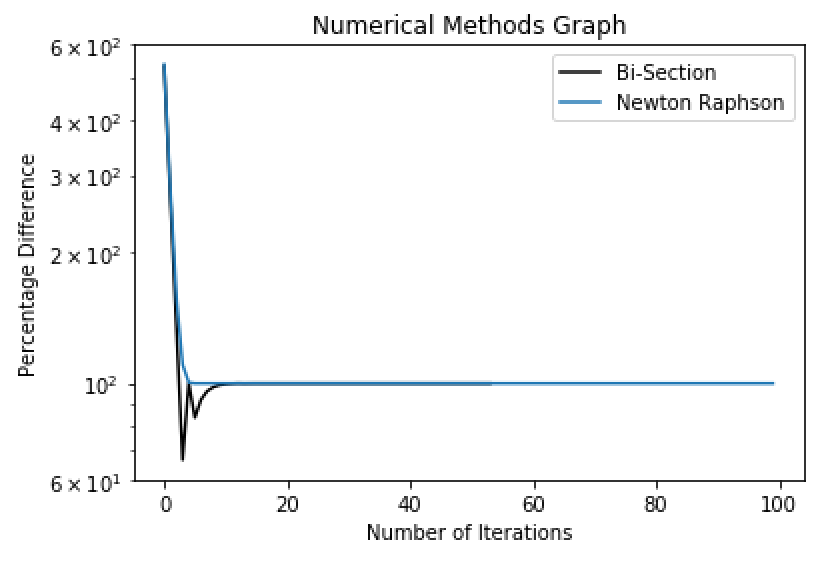
\includegraphics[scale=0.8]{Numerical_Methods_Graph.png}
\caption{Plots of Bi-Section and Newton Raphson} {methods of finding the square root of 114.114.}
\label{Numerical Methods Graph}
\end{figure}

In analysis of the graph the Newton Raphson method in \cref{S5} shows 
a faster answer with less iterations done compared to the Bi-Section method in \cref{S4}, this is also proven by the less amount of error percentage in each iteration. Even though both the Bi-Section and Newton Raphson methods both share the same goal the process of reaching that goal is completely different, the Newton Raphson method halves the estimated value and keeps halving it until the error percentage associated with it, where as the Bi- Section method uses more of a trial and error approach, wilding guessing estimated values until the error percentage is equal to zero. \\

This experiment between both root finding methods has proven though both can fulfill the same goal, one is less time consuming than the other, but when writing the script for Newton Raphson, it is more sensitive and high maintenance compared to the Bi-Section. 


%-----------------------------------------------------------------------
%-----------------------------------------------------------------------
%	PLOTTING SCRIPT
%-----------------------------------------------------------------------
%-----------------------------------------------------------------------

\section{Plotting Script}
\label{S3}

This section contains the written plotting script of code for the completion of this assessment \cite{Numerical_Methods}, the varible outputs are displayed in the \cref{Numerical Methods Graph}.

\begin{minted}[bgcolor=AliceBlue]{python3}

import csv
import numpy as np
import matplotlib.pylab as plt


def getColumn(filename, column):
    results = csv.reader(open(filename), dialect='excel')
    return [result[column] for result in results]
# This allows the script to identify nad isolate columns in data
# files, as specified data file have 3 columns and this only 
# having need of 2 of them.

BI_Its = getColumn("Bi-Section Script.csv",0) 
BI_Per = getColumn("Bi-Section Script.csv",2)
# This section allows the script to input data from an external 
# source, the 0 and 2 are to isolate the data from 2 specific
# columns i.e. number of iteration and percentage difference.


NR_Its = getColumn("Newton Raphson Script.csv",0)
NR_Per = getColumn("Newton Raphson Script.csv",2)
# This section allows the script to input data from an external 
# source, the 0 and 2 are to isolate the data from 2 specific 
# columns i.e. number of iteration and percentage difference.

plt.semilogy(BI_Its,BI_Per, 'k', label='Bi-Section')
plt.semilogy(NR_Its, NR_Per, label='Newton Raphson')
# Plots both sets of data together on the same graph.

plt.xlabel('Number of Iterations')
plt.ylabel('Percentage Difference')
plt.title('Numerical Methods Graph')
# Labels to identify both axes.

plt.legend()
# To identify which sets of data belong to which script.

plt.savefig('Numerical Methods Graph.png')
# Externally saving the png image on its own for further 
# analysis.

plt.show()

\end{minted}

%-----------------------------------------------------------------------
%-----------------------------------------------------------------------
%	BI-SECTION SCRIPT
%-----------------------------------------------------------------------
%-----------------------------------------------------------------------

\section{Bi-Section Script}
\label{S4}

This section contains the written Bi-Secion script of code for the completion of this assessment \cite{Numerical_Methods}, the varible outputs are displayed in the \cref{Numerical Methods Graph}.

\begin{minted}[bgcolor=AliceBlue]{python3}

import numpy as np
import time as time

f = open('Bi-Section Script.csv', 'w')
# Where f is the output file for the values made by the 
# following code.

a = float(input("Enter Value to be Square Rooted: "))
# a is a use typed input and is the value to be square rooted.

n = 100
# n is maximum number of iterations to be conducted.

x_high = a 
x_low = x_high - x_high
x_mid = a/2
dx = x_high/4

start = time.clock()
# This line of code measures the time taken to calculate the 
# values.

for i in range(n):
    k = x_mid**2 - a
# k is a constant that needs to be as close to 0 as possible, 
# the equation is in reference to the workshop 10 guide.
    
    Per_err = (x_mid / np.sqrt(a)) * 100
# This equation defines the percentage of error of the 
# estimated value.

    print("Iteration No.",i)
    print("Estimate Value for", i, "=", x_mid)
    print("Percentage Error for", i, "=", Per_err, "%")
    print(k)
    print(" ")

# In the previous 5 lines, when displayed, the values for: 
# iteration, estimated value, percentage error and the 
# constant that needs to be as close to 0 as possible , then 
# follow by a gap to allow the calculated values to be 
# easily read.
    if k > 0:
        x_mid = x_mid - dx
        
    elif k < 0:
        x_mid = x_mid + dx
    
    dx = dx/2
        
    if -1e-16 < k and k < 1e-16:
        break
    
    f.write("{0}, {1}, {2}\n".format(str(i), str(x_mid), str(Per_err)))
# Saving all data to and external csv file for 
# further analysis

end = time.clock()
time = end - start

print("Enter Value to be Square Rooted =", a)
print("Final Square Rooted Value =", x_mid)
print("Total Number of Iterations =", i)
print("Percentage Error =", Per_err)
print("Total Time (In Seconds) =", time)
# Telling the script to show the user specfied data.

\end{minted}
%-----------------------------------------------------------------------
%-----------------------------------------------------------------------
%	NEWTON RAPHSON SCRIPT
%-----------------------------------------------------------------------
%-----------------------------------------------------------------------

\section{Newton Raphson Script}
\label{S5}

This section contains the written Newton Raphson script of code for the completion of this assessment \cite{Numerical_Methods}, the varible outputs are displayed in the \cref{Numerical Methods Graph}.

\begin{minted}[bgcolor=AliceBlue]{python3}

import numpy as np
import time as time

it = 0
f = open('Newton Raphson Script.c', 'w')
# Where f is the output file for the values made by the 
# following code.

n = 100
diff = 100

num = float(input("Enter Value to be Square Rooted: "))
# num is a use typed input and is the value to be square rooted.

start = time.clock()

mid = num
    
for i in range(n):
    x = mid - ((mid**2 - num)/(2*mid))
    if diff != 0:
        it = i
        diff = (((np.sqrt(num)-x)/np.sqrt(num))*100)
        mid = x
        f.write("{0}, {1}, {2}\n".format(str(it), str(mid), str(diff)))
        
    else:
        break
    
f.close()
end = time.clock()
time = end - start
# This line of code measures the time taken to calculate the 
# values.

print("The inputted number was", num, ".")
print("The root of", num, "is", x, ".")
print("This process took the program", time, "seconds.")
print("this took", it, "iterations to find")
print("Per iteration, this took", time/it, "s.")
# Telling the script to show the user specfied data.

\end{minted}

%------------------------------------------------------------------------
%	REFERENCES
%------------------------------------------------------------------------

\bibliographystyle{plain}
\bibliography{mybib.bib}

%------------------------------------------------------------------------

\pagebreak
\inputminted[breaklines]{tex}{main.tex}
\pagebreak
\inputminted[breaklines]{tex}{mybib.bib}
\end{document}